\documentclass[12pt,a4paper]{article}
\usepackage[utf8]{vietnam}
\usepackage{amsmath,amssymb,amsfonts,mathrsfs}
\usepackage[left=1.5cm,right=1.5cm,top=2cm,bottom=2cm,headheight=17pt]{geometry}
\usepackage{enumitem}
\usepackage{array}
\usepackage{graphicx}
\usepackage{tikz}
\usetikzlibrary{arrows.meta,calc,patterns}
\usepackage{fancyhdr}

\pagestyle{fancy}
\fancyhf{}
\lhead{\small\textbf{HƯỚNG TỚI THPTQG 2027}}
\rhead{\small\textit{Người biên soạn: Dương Gia Bảo}}
\rfoot{\small Trang \thepage}
\renewcommand{\headrulewidth}{0.4pt}

\begin{document}

\noindent
\begin{minipage}[t]{0.40\textwidth}
    \centering
    \textbf{HƯỚNG TỚI THPTQG 2027}\\[-2pt]
    \rule{3.2cm}{0.6pt}\\[4pt]
    \textbf{ĐỀ CHÍNH THỨC}
\end{minipage}\hfill
\begin{minipage}[t]{0.58\textwidth}
    \centering
    \textbf{ĐỀ THI KHẢO SÁT CHẤT LƯỢNG}\\
    \textbf{ĐỀ SỐ 14}\\
    \textbf{Môn thi: TOÁN}\\
    \textit{\small Thời gian làm bài: 90 phút, không kể thời gian phát đề}
\end{minipage}

\vspace{0.2cm}
\noindent
\begin{minipage}[b]{0.78\textwidth}
    \textbf{Họ và tên:}\dotfill\textbf{SBD:}\makebox[3.5cm]{\dotfill}
\end{minipage}\hfill
\begin{minipage}[b]{0.20\textwidth}
    \hfill
    \setlength{\fboxrule}{0.8pt}%
    \fbox{\begin{minipage}{2.3cm}
        \centering
        \textbf{\small Mã đề thi}\\
        \textbf{0014}
    \end{minipage}}
\end{minipage}
\vspace{0.2cm}

% ==========================================
% PHẦN I
% ==========================================
\section*{\large PHẦN I. CÂU TRẮC NGHIỆM NHIỀU PHƯƠNG ÁN LỰA CHỌN}
\textit{Thí sinh trả lời từ câu 1 đến câu 12. Mỗi câu hỏi thí sinh chỉ chọn một phương án. Mỗi câu trả lời đúng được 0,25 điểm.}

\begin{enumerate}[label=\textbf{Câu \arabic*:}, leftmargin=*]

\item Số đường tiệm cận (gồm tiệm cận đứng và tiệm cận ngang) của đồ thị hàm số $y = \dfrac{x^2 - 1}{x^2 - 4x + 3}$ là
\begin{enumerate}[label=\Alph*.]
    \item $1$.
    \item $2$.
    \item $3$.
    \item $4$.
\end{enumerate}

\item Số nghiệm nguyên của bất phương trình $2^{x^2 - 3x} < 16$ là
\begin{enumerate}[label=\Alph*.]
    \item $2$.
    \item $3$.
    \item $5$.
    \item $4$.
\end{enumerate}

\item Giá trị của tích phân $\displaystyle \int_0^1 x e^x\,\mathrm{d}x$ bằng
\begin{enumerate}[label=\Alph*.]
    \item $1$.
    \item $e$.
    \item $e - 1$.
    \item $2$.
\end{enumerate}

\item Trong không gian $Oxyz$, mặt phẳng đi qua ba điểm $A(1; 0; 0)$, $B(0; 2; 0)$, $C(0; 0; 3)$ có phương trình là
\begin{enumerate}[label=\Alph*.]
    \item $x + 2y + 3z - 6 = 0$.
    \item $6x + 3y + 2z + 6 = 0$.
    \item $6x + 3y + 2z - 6 = 0$.
    \item $2x + 3y + 6z - 6 = 0$.
\end{enumerate}

\item Gieo đồng thời hai con xúc xắc cân đối và đồng chất. Biết rằng có ít nhất một con xúc xắc xuất hiện mặt $6$ chấm, xác suất để tổng số chấm trên hai con xúc xắc bằng $8$ là
\begin{enumerate}[label=\Alph*.]
    \item $\dfrac{5}{36}$.
    \item $\dfrac{1}{6}$.
    \item $\dfrac{1}{11}$.
    \item $\dfrac{2}{11}$.
\end{enumerate}

\item Một mẫu số liệu ghép nhóm gồm $20$ giá trị có bảng tần số như sau:
\begin{center}
\begin{tabular}{|c|c|c|c|}
\hline
\textbf{Nhóm} & $[10; 20)$ & $[20; 30)$ & $[30; 40)$ \\ \hline
\textbf{Tần số} & 5 & 10 & 5 \\ \hline
\end{tabular}
\end{center}
Phương sai của mẫu số liệu ghép nhóm trên bằng
\begin{enumerate}[label=\Alph*.]
    \item $25$.
    \item $50$.
    \item $100$.
    \item $7{,}07$.
\end{enumerate}

\item Thể tích của khối tứ diện đều có cạnh bằng $a$ là
\begin{enumerate}[label=\Alph*.]
    \item $\dfrac{a^3\sqrt{2}}{12}$.
    \item $\dfrac{a^3\sqrt{3}}{12}$.
    \item $\dfrac{a^3}{6}$.
    \item $\dfrac{a^3\sqrt{2}}{4}$.
\end{enumerate}

\item Cho cấp số cộng $(u_n)$ có số hạng đầu $u_1 = 5$ và công sai $d = 3$. Tổng $20$ số hạng đầu tiên của cấp số cộng bằng
\begin{enumerate}[label=\Alph*.]
    \item $590$.
    \item $650$.
    \item $670$.
    \item $700$.
\end{enumerate}

\item Dân số của một quốc gia hiện nay là $90$ triệu người, tốc độ tăng dân số là $1{,}2\%$/năm. Nếu tốc độ tăng dân số được giữ nguyên thì sau $10$ năm, dân số quốc gia đó xấp xỉ bao nhiêu triệu người? (làm tròn đến hàng phần mười)
\begin{enumerate}[label=\Alph*.]
    \item $101{,}4$.
    \item $100{,}8$.
    \item $102{,}6$.
    \item $110{,}0$.
\end{enumerate}

\item Trong không gian $Oxyz$, cho hai vectơ $\vec{a} = (1; 1; 0)$ và $\vec{b} = (0; 1; 1)$. Góc giữa hai vectơ $\vec{a}$ và $\vec{b}$ bằng
\begin{enumerate}[label=\Alph*.]
    \item $30^\circ$.
    \item $45^\circ$.
    \item $90^\circ$.
    \item $60^\circ$.
\end{enumerate}

\item Một người có $200\text{ m}$ hàng rào, muốn rào một mảnh vườn hình chữ nhật dựa vào một bức tường thẳng (không cần rào phía tường). Diện tích lớn nhất của mảnh vườn có thể rào được bằng bao nhiêu mét vuông?
\begin{enumerate}[label=\Alph*.]
    \item $2500$.
    \item $4000$.
    \item $5000$.
    \item $10000$.
\end{enumerate}

\item Thể tích của khối cầu có bán kính $R = 3$ bằng
\begin{enumerate}[label=\Alph*.]
    \item $12\pi$.
    \item $36\pi$.
    \item $27\pi$.
    \item $108\pi$.
\end{enumerate}

\end{enumerate}

% ==========================================
% PHẦN II
% ==========================================
\vspace{0.4cm}
\section*{\large PHẦN II. CÂU TRẮC NGHIỆM ĐÚNG SAI}
\textit{Thí sinh trả lời từ câu 1 đến câu 4. Trong mỗi ý \textbf{a)}, \textbf{b)}, \textbf{c)}, \textbf{d)} ở mỗi câu, thí sinh chọn đúng hoặc sai.}

\begin{enumerate}[label=\textbf{Câu \arabic*:}, leftmargin=*]

\item \begin{minipage}[t]{0.55\linewidth}
Nhà máy $A$ nằm trên bờ biển. Hòn đảo $B$ cách bờ biển $4\text{ km}$; hình chiếu vuông góc của $B$ lên bờ là điểm $H$ cách $A$ một khoảng $10\text{ km}$. Người ta kéo cáp điện từ $A$ ra đảo $B$ như sau: kéo dọc bờ biển từ $A$ đến điểm $M$ cách $A$ một đoạn $t$ ($\text{km}$, $0 \le t \le 10$), sau đó kéo dưới biển từ $M$ thẳng đến $B$. Chi phí kéo cáp trên bờ là $3$ triệu đồng/km, dưới biển là $5$ triệu đồng/km.
\begin{enumerate}[label=\textbf{\alph*)}]
    \item Tổng chi phí kéo cáp là $f(t) = 3t + 5\sqrt{16 + (10 - t)^2}$ (triệu đồng).
    \item Nếu kéo cáp thẳng từ $A$ đến $B$ hoàn toàn dưới biển thì chi phí bằng $50$ triệu đồng.
    \item Tổng chi phí nhỏ nhất đạt được khi $t = 7\text{ km}$.
    \item Tổng chi phí nhỏ nhất bằng $46$ triệu đồng.
\end{enumerate}
\end{minipage}\hfill
\begin{minipage}[t]{0.42\linewidth}
\vspace{-0.4\baselineskip}
\centering
\resizebox{\linewidth}{!}{%
\begin{tikzpicture}[>=Stealth, x=0.6cm, y=0.6cm, line join=round, line cap=round]
    % Vùng biển phía trên bờ
    \fill[blue!7] (-1.4,0) rectangle (11.4,5.6);
    \draw[very thick] (-1.4,0) -- (11.4,0);
    \node[right, font=\footnotesize] at (-1.4,4.9) {biển};
    \node[right, font=\footnotesize] at (2.2,-0.8) {đất liền};

    % Các điểm
    \coordinate (H) at (0,0);
    \coordinate (B) at (0,4);
    \coordinate (M) at (7,0);
    \coordinate (A) at (10,0);

    % Cáp trên bờ A -> M và dưới biển M -> B
    \draw[very thick, orange!85!black] (A) -- (M);
    \draw[very thick, blue!70!black] (M) -- (B);
    \draw[dashed, thick, gray!80!black] (H) -- (B);
    \draw[thin] (0,0.45) -- (0.45,0.45) -- (0.45,0);

    % Điểm mốc
    \filldraw[fill=orange!80!red, draw=black, thick] (A) circle (2.2pt) node[below, fill=white, inner sep=1.2pt] {$A$};
    \filldraw[fill=white, draw=black, thick] (M) circle (2.2pt) node[below, fill=white, inner sep=1.2pt] {$M$};
    \filldraw[fill=white, draw=black, thick] (H) circle (2.2pt) node[below, fill=white, inner sep=1.2pt] {$H$};
    \filldraw[fill=blue!25, draw=black, thick] (B) circle (2.6pt) node[above right, fill=white, inner sep=1.2pt] {$B$};
\end{tikzpicture}%
}
\end{minipage}

\item Trong không gian $Oxyz$, cho mặt cầu $(S): x^2 + y^2 + z^2 - 2x + 4y - 4z - 16 = 0$ và mặt phẳng $(P): 2x - 2y + z + 4 = 0$.
\begin{enumerate}[label=\textbf{\alph*)}]
    \item Mặt cầu $(S)$ có tâm $I(1; -2; 2)$.
    \item Mặt cầu $(S)$ có bán kính $R = 5$.
    \item Mặt phẳng $(P)$ tiếp xúc với mặt cầu $(S)$.
    \item Mặt phẳng $(P)$ cắt mặt cầu $(S)$ theo giao tuyến là đường tròn có diện tích bằng $16\pi$.
\end{enumerate}

\item \begin{minipage}[t]{0.55\linewidth}
Một nhà máy lắp ráp nhận linh kiện từ ba nhà cung cấp $A$, $B$, $C$ với tỉ lệ lần lượt là $50\%$, $30\%$, $20\%$ tổng số linh kiện. Tỉ lệ linh kiện lỗi của ba nhà cung cấp lần lượt là $1\%$, $2\%$, $3\%$. Chọn ngẫu nhiên một linh kiện.
\begin{enumerate}[label=\textbf{\alph*)}]
    \item Xác suất để linh kiện được chọn bị lỗi bằng $0{,}02$.
    \item Nếu linh kiện được chọn bị lỗi thì xác suất để nó do nhà cung cấp $A$ cung cấp nhỏ hơn $30\%$.
    \item Nếu linh kiện được chọn bị lỗi thì xác suất để nó do nhà cung cấp $B$ cung cấp bằng xác suất để nó do nhà cung cấp $C$ cung cấp.
    \item Chọn ngẫu nhiên và độc lập hai linh kiện, xác suất để có ít nhất một linh kiện bị lỗi bằng $0{,}0340$.
\end{enumerate}
\end{minipage}\hfill
\begin{minipage}[t]{0.42\linewidth}
\vspace{-0.4\baselineskip}
\centering
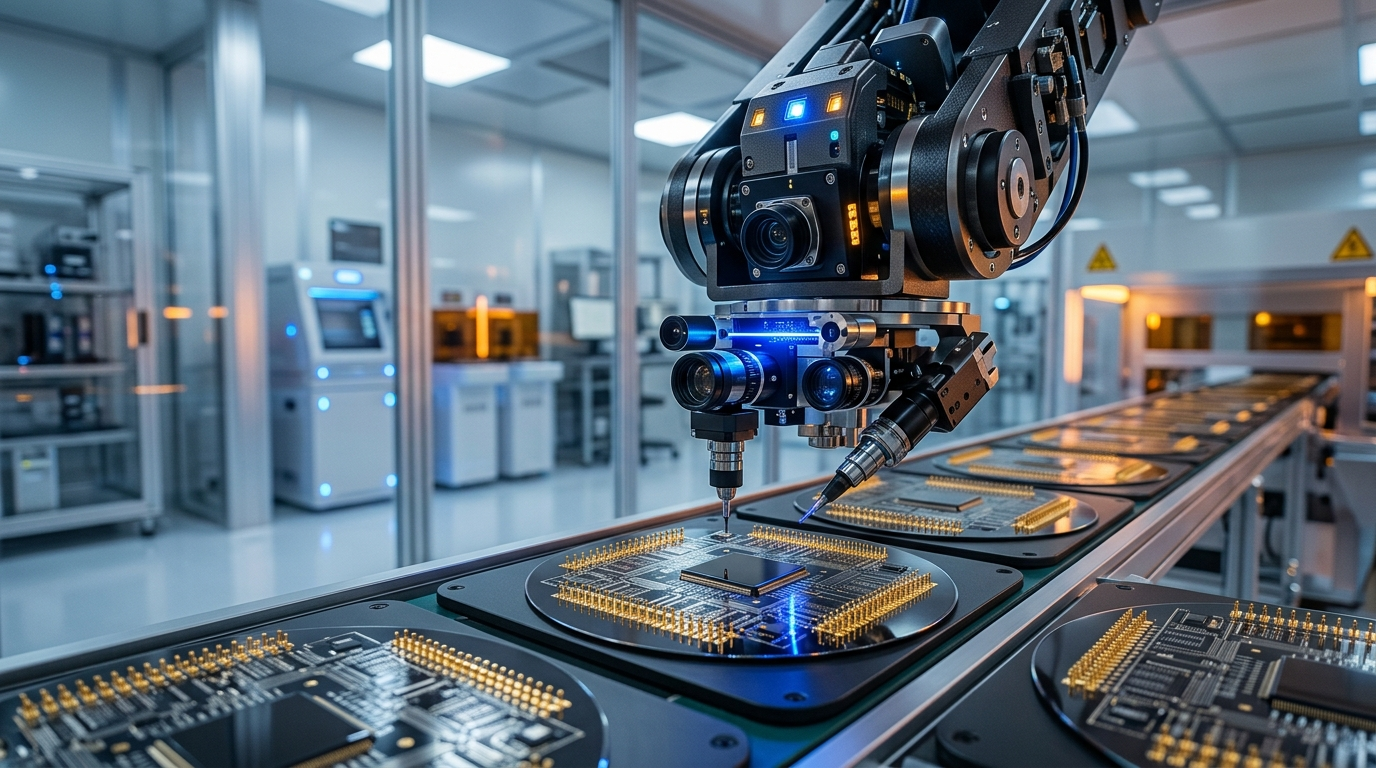
\includegraphics[width=\linewidth, keepaspectratio]{images/de14_chip_factory.jpg}
\end{minipage}

\item Một chất điểm chuyển động thẳng với vận tốc $v(t) = 6t - t^2$ (đơn vị: m/s), $t \ge 0$ tính bằng giây.
\begin{enumerate}[label=\textbf{\alph*)}]
    \item Vận tốc của chất điểm đạt giá trị lớn nhất tại thời điểm $t = 6\text{ s}$.
    \item Quãng đường chất điểm đi được từ thời điểm $t = 0$ đến $t = 6\text{ s}$ bằng $36\text{ m}$.
    \item Gia tốc của chất điểm tại thời điểm $t = 4\text{ s}$ bằng $2\text{ m/s}^2$.
    \item Quãng đường chất điểm đi được trong $3$ giây đầu tiên bằng $18\text{ m}$.
\end{enumerate}

\end{enumerate}

% ==========================================
% PHẦN III
% ==========================================
\vspace{0.4cm}
\section*{\large PHẦN III. CÂU TRẮC NGHIỆM TRẢ LỜI NGẮN}
\textit{Thí sinh trả lời từ câu 1 đến câu 6. Mỗi câu trả lời đúng được 0,5 điểm.}

\begin{enumerate}[label=\textbf{Câu \arabic*:}, leftmargin=*]

\item Cho hình chóp $S.ABCD$ có đáy $ABCD$ là hình vuông, cạnh bên $SA$ vuông góc với mặt phẳng đáy và $SA = AB$. Số đo (tính theo độ) của góc giữa hai mặt phẳng $(SBC)$ và $(SCD)$ bằng bao nhiêu?

\item \begin{minipage}[t]{0.55\linewidth}
Gọi $(H)$ là hình phẳng giới hạn bởi đồ thị hàm số $y = x^2$ và đường thẳng $y = x$ (phần gạch chéo trong hình vẽ bên). Quay hình $(H)$ quanh trục $Ox$ ta được một khối tròn xoay có thể tích $V$. Tính $V$ (kết quả làm tròn đến hàng phần trăm).
\end{minipage}\hfill
\begin{minipage}[t]{0.42\linewidth}
\vspace{-0.4\baselineskip}
\centering
\resizebox{0.85\linewidth}{!}{%
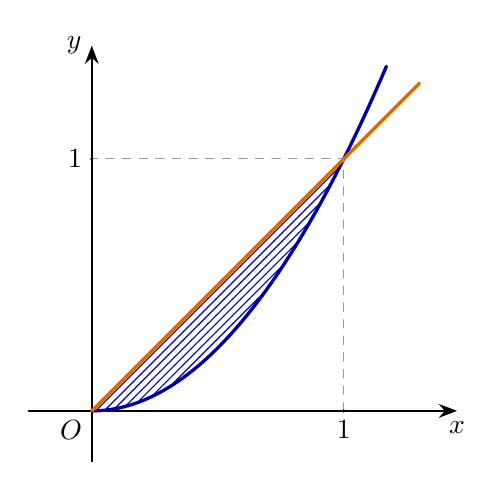
\begin{tikzpicture}[>=Stealth, x=3.2cm, y=3.2cm, line join=round, line cap=round]
    % Trục tọa độ
    \draw[->, thick] (-0.25,0) -- (1.45,0) node[below] {$x$};
    \draw[->, thick] (0,-0.2) -- (0,1.45) node[left] {$y$};
    \node[below left] at (0,0) {$O$};

    % Miền gạch chéo giữa y = x và y = x^2
    \fill[pattern=north east lines, pattern color=blue!75!black, domain=0:1, samples=40]
        plot (\x, {\x*\x}) -- cycle;

    % Hai đường
    \draw[very thick, blue!65!black, domain=0:1.17, samples=50] plot (\x, {\x*\x});
    \draw[very thick, orange!85!black] (0,0) -- (1.3,1.3);

    % Mốc
    \draw[dashed, thin, gray!80] (1,0) -- (1,1) -- (0,1);
    \fill (1,0) circle (0.6pt) node[below] {$1$};
    \fill (0,1) circle (0.6pt) node[left] {$1$};
\end{tikzpicture}%
}
\end{minipage}

\item \begin{minipage}[t]{0.58\linewidth}
Một hành lang hình chữ L gồm hai đoạn vuông góc với nhau có chiều rộng lần lượt là $8\text{ m}$ và $1\text{ m}$. Người ta muốn khiêng một thanh cứng thẳng (coi như một đoạn thẳng, bỏ qua bề dày) đi theo phương nằm ngang qua chỗ rẽ của hành lang. Chiều dài lớn nhất của thanh có thể khiêng qua chỗ rẽ đó bằng bao nhiêu mét? (kết quả làm tròn đến hàng phần mười).
\end{minipage}\hfill
\begin{minipage}[t]{0.38\linewidth}
\vspace{-0.4\baselineskip}
\centering
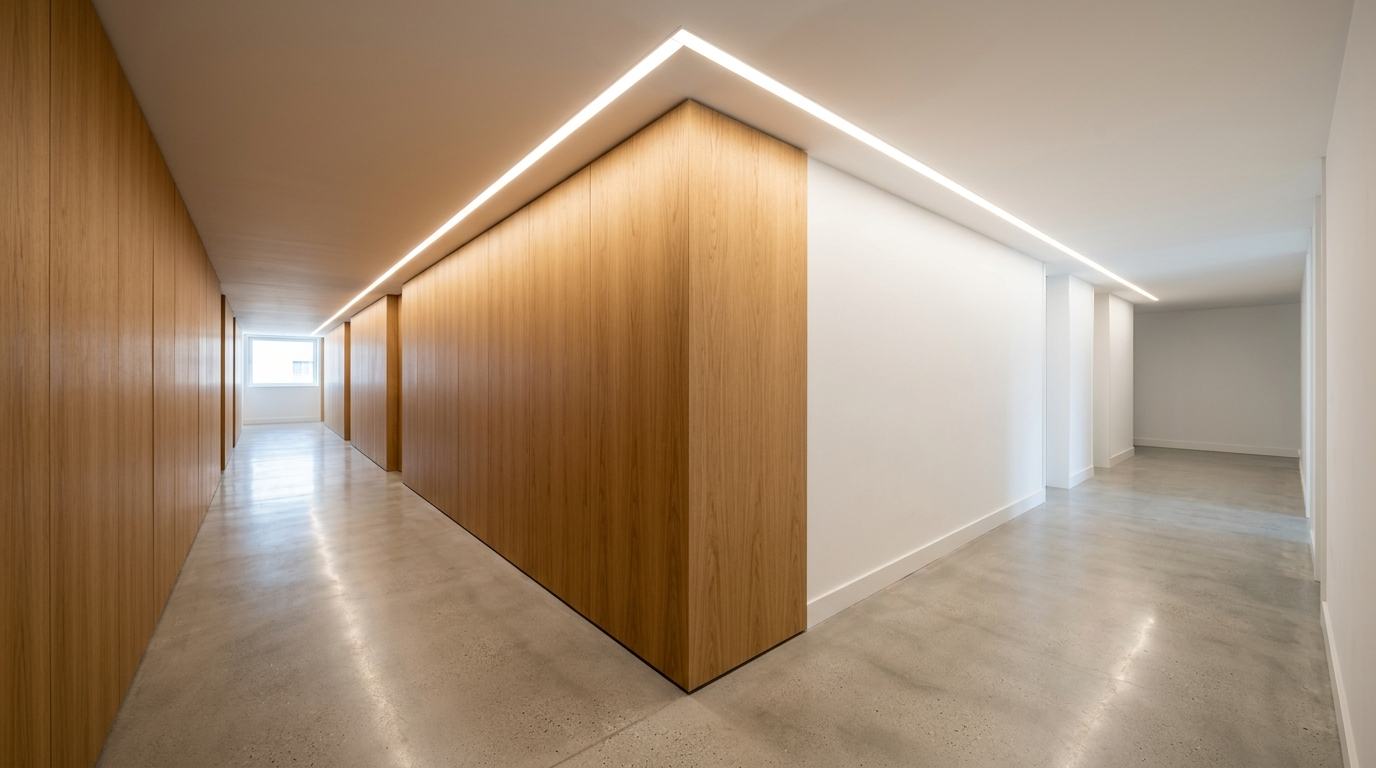
\includegraphics[width=\linewidth, keepaspectratio]{images/de14_corridor_turn.jpg}
\end{minipage}

\item Trong không gian $Oxyz$, một tia sáng phát ra từ nguồn sáng $A(1; 2; 3)$ chiếu tới một gương phẳng có phương trình $(P): 2x + y - 2z + 11 = 0$. Gọi $A'(a; b; c)$ là ảnh của điểm $A$ qua gương $(P)$ (tức là điểm đối xứng của $A$ qua mặt phẳng $(P)$). Tính $a + b + c$.

\item \begin{minipage}[t]{0.55\linewidth}
Trong loạt đá luân lưu quyết định, siêu sao Cristiano Ronaldo thực hiện $6$ quả sút luân lưu $11\text{m}$. Giả sử các lần sút là độc lập với nhau và xác suất sút thành công ở mỗi lần của anh đều bằng $0{,}9$. Xác suất để Cristiano Ronaldo sút thành công ít nhất $5$ quả bằng bao nhiêu? (kết quả làm tròn đến hàng phần trăm).
\end{minipage}\hfill
\begin{minipage}[t]{0.42\linewidth}
\vspace{-0.4\baselineskip}
\centering

\includegraphics[width=\linewidth, keepaspectratio]{cr7_siuuu_alnassr.png}
\end{minipage}

\item Một quả bóng bay hình cầu được bơm khí sao cho thể tích của nó tăng với tốc độ $18\pi\ (\text{cm}^3/\text{s})$. Tại thời điểm bán kính của quả bóng bằng $3\text{ cm}$, bán kính của quả bóng tăng với tốc độ bao nhiêu xăng-ti-mét trên giây?

\end{enumerate}

% ==========================================
% BẢNG ĐÁP ÁN TỔNG HỢP (BẮT BUỘC TRANG MỚI)
% ==========================================
\newpage
\begin{center}
    {\Large\textbf{BẢNG ĐÁP ÁN TỔNG HỢP}}\\[4pt]
    \textbf{ĐỀ SỐ 14 - MÔN: TOÁN}
\end{center}
\vspace{0.3cm}

\noindent\textbf{\large PHẦN I. CÂU TRẮC NGHIỆM NHIỀU PHƯƠNG ÁN LỰA CHỌN}
\begin{center}
\renewcommand{\arraystretch}{1.25}
\begin{tabular}{|c|c|c|c|c|c|c|c|c|c|c|c|}
\hline
\textbf{1} & \textbf{2} & \textbf{3} & \textbf{4} & \textbf{5} & \textbf{6} & \textbf{7} & \textbf{8} & \textbf{9} & \textbf{10} & \textbf{11} & \textbf{12} \\ \hline
\textbf{B} & \textbf{D} & \textbf{A} & \textbf{C} & \textbf{D} & \textbf{B} & \textbf{A} & \textbf{C} & \textbf{A} & \textbf{D} & \textbf{C} & \textbf{B} \\ \hline
\end{tabular}
\end{center}

\vspace{0.3cm}
\noindent\textbf{\large PHẦN II. CÂU TRẮC NGHIỆM ĐÚNG SAI}
\begin{center}
\renewcommand{\arraystretch}{1.25}
\begin{tabular}{|c|c|c|c|c|}
\hline
\textbf{Câu} & \textbf{Ý a)} & \textbf{Ý b)} & \textbf{Ý c)} & \textbf{Ý d)} \\ \hline
\textbf{Câu 1} & Đ & S & Đ & Đ \\ \hline
\textbf{Câu 2} & Đ & Đ & S & S \\ \hline
\textbf{Câu 3} & S & Đ & Đ & S \\ \hline
\textbf{Câu 4} & S & Đ & S & Đ \\ \hline
\end{tabular}
\end{center}

\vspace{0.3cm}
\noindent\textbf{\large PHẦN III. CÂU TRẮC NGHIỆM TRẢ LỜI NGẮN}
\begin{center}
\renewcommand{\arraystretch}{1.25}
\begin{tabular}{|c|c|c|c|c|c|}
\hline
\textbf{Câu 1} & \textbf{Câu 2} & \textbf{Câu 3} & \textbf{Câu 4} & \textbf{Câu 5} & \textbf{Câu 6} \\ \hline
60 & 0,42 & 11,2 & 4 & 0,89 & 0,5 \\ \hline
\end{tabular}
\end{center}

% ==========================================
% HƯỚNG DẪN GIẢI CHI TIẾT
% ==========================================
\newpage
\begin{center}
    {\Large\textbf{HƯỚNG DẪN GIẢI CHI TIẾT}}\\[4pt]
    \textbf{ĐỀ SỐ 14 - MÔN: TOÁN}
\end{center}
\vspace{0.3cm}

\section*{\large PHẦN I. CÂU TRẮC NGHIỆM NHIỀU PHƯƠNG ÁN LỰA CHỌN}

\noindent\textbf{Câu 1.} Ta có $y = \dfrac{(x - 1)(x + 1)}{(x - 1)(x - 3)} = \dfrac{x + 1}{x - 3}$ với $x \ne 1$, $x \ne 3$.\\
$\lim\limits_{x \to 3^+} y = +\infty$ nên $x = 3$ là tiệm cận đứng. Tại $x = 1$: $\lim\limits_{x \to 1} y = \dfrac{2}{-2} = -1$ hữu hạn nên $x = 1$ không phải tiệm cận đứng.\\
$\lim\limits_{x \to \pm\infty} y = 1$ nên $y = 1$ là tiệm cận ngang. Vậy đồ thị có $2$ đường tiệm cận.\\
\textbf{Chọn B.}

\vspace{0.25cm}
\noindent\textbf{Câu 2.} $2^{x^2 - 3x} < 2^4 \iff x^2 - 3x - 4 < 0 \iff -1 < x < 4$. Các nghiệm nguyên là $0; 1; 2; 3$, tức là $4$ nghiệm.\\
\textbf{Chọn D.}

\vspace{0.25cm}
\noindent\textbf{Câu 3.} Tích phân từng phần với $u = x$, $\mathrm{d}v = e^x\mathrm{d}x$:
\[
\int_0^1 x e^x\,\mathrm{d}x = \Big[x e^x\Big]_0^1 - \int_0^1 e^x\,\mathrm{d}x = e - (e - 1) = 1.
\]
\textbf{Chọn A.}

\vspace{0.25cm}
\noindent\textbf{Câu 4.} Mặt phẳng cắt các trục tọa độ tại $A(1; 0; 0)$, $B(0; 2; 0)$, $C(0; 0; 3)$ có phương trình theo đoạn chắn
\[
\dfrac{x}{1} + \dfrac{y}{2} + \dfrac{z}{3} = 1 \iff 6x + 3y + 2z - 6 = 0.
\]
\textbf{Chọn C.}

\vspace{0.25cm}
\noindent\textbf{Câu 5.} Gọi $A$: "có ít nhất một con xúc xắc ra mặt $6$ chấm", $B$: "tổng số chấm bằng $8$".\\
$n(A) = 36 - 25 = 11$. $A \cap B$ gồm các kết quả $(2; 6)$ và $(6; 2)$ nên $n(A \cap B) = 2$.
\[
P(B|A) = \dfrac{n(A \cap B)}{n(A)} = \dfrac{2}{11}.
\]
\textbf{Chọn D.}

\vspace{0.25cm}
\noindent\textbf{Câu 6.} Giá trị đại diện: $15; 25; 35$. Số trung bình $\overline{x} = \dfrac{5\cdot 15 + 10\cdot 25 + 5\cdot 35}{20} = 25$.
\[
s^2 = \dfrac{5(15 - 25)^2 + 10(25 - 25)^2 + 5(35 - 25)^2}{20} = \dfrac{500 + 0 + 500}{20} = 50.
\]
\textbf{Chọn B.}

\vspace{0.25cm}
\noindent\textbf{Câu 7.} Tứ diện đều cạnh $a$ có diện tích đáy $S = \dfrac{a^2\sqrt{3}}{4}$ và chiều cao $h = \dfrac{a\sqrt{6}}{3}$. Do đó
\[
V = \dfrac{1}{3}Sh = \dfrac{1}{3}\cdot\dfrac{a^2\sqrt{3}}{4}\cdot\dfrac{a\sqrt{6}}{3} = \dfrac{a^3\sqrt{2}}{12}.
\]
\textbf{Chọn A.}

\vspace{0.25cm}
\noindent\textbf{Câu 8.}
\[
S_{20} = \dfrac{20}{2}\left[2u_1 + 19d\right] = 10\,(10 + 57) = 670.
\]
\textbf{Chọn C.}

\vspace{0.25cm}
\noindent\textbf{Câu 9.} Dân số sau $10$ năm là $90\cdot (1 + 0{,}012)^{10} = 90\cdot 1{,}012^{10} \approx 90\cdot 1{,}1267 \approx 101{,}4$ (triệu người).\\
\textbf{Chọn A.}

\vspace{0.25cm}
\noindent\textbf{Câu 10.}
\[
\cos(\vec{a}, \vec{b}) = \dfrac{\vec{a}\cdot\vec{b}}{|\vec{a}||\vec{b}|} = \dfrac{1\cdot 0 + 1\cdot 1 + 0\cdot 1}{\sqrt{2}\cdot\sqrt{2}} = \dfrac{1}{2} \implies (\vec{a}, \vec{b}) = 60^\circ.
\]
\textbf{Chọn D.}

\vspace{0.25cm}
\noindent\textbf{Câu 11.} Gọi $y$ (m) là độ dài mỗi cạnh vuông góc với tường ($0 < y < 100$), cạnh song song với tường dài $200 - 2y$. Diện tích mảnh vườn:
\[
S(y) = y(200 - 2y) = -2y^2 + 200y.
\]
$S$ đạt giá trị lớn nhất tại $y = 50$ và $S_{\max} = 50\cdot 100 = 5000\text{ m}^2$.\\
\textbf{Chọn C.}

\vspace{0.25cm}
\noindent\textbf{Câu 12.}
\[
V = \dfrac{4}{3}\pi R^3 = \dfrac{4}{3}\pi\cdot 27 = 36\pi.
\]
\textbf{Chọn B.}

% ==========================================
\vspace{0.4cm}
\section*{\large PHẦN II. CÂU TRẮC NGHIỆM ĐÚNG SAI}

\noindent\textbf{Câu 1.} Ta có $AM = t$, $MH = 10 - t$, $MB = \sqrt{BH^2 + MH^2} = \sqrt{16 + (10 - t)^2}$. Chi phí:
\[
f(t) = 3t + 5\sqrt{16 + (10 - t)^2}, \quad t \in [0; 10].
\]
$\implies$ \textbf{a) ĐÚNG.}

Kéo thẳng từ $A$ đến $B$ dưới biển ứng với $t = 0$: $f(0) = 5\sqrt{16 + 100} = 5\sqrt{116} \approx 53{,}85 \ne 50$.\\
$\implies$ \textbf{b) SAI.}

Đạo hàm: $f'(t) = 3 - \dfrac{5(10 - t)}{\sqrt{16 + (10 - t)^2}}$. Đặt $u = 10 - t$, $f'(t) = 0 \iff 3\sqrt{16 + u^2} = 5u \iff 9(16 + u^2) = 25u^2 \iff u^2 = 9 \iff u = 3$ (do $u > 0$).\\
Suy ra $t = 7$. Ta có $f(0) \approx 53{,}85$, $f(7) = 21 + 5\cdot 5 = 46$, $f(10) = 30 + 20 = 50$ nên $f$ đạt giá trị nhỏ nhất tại $t = 7$.\\
$\implies$ \textbf{c) ĐÚNG}, \textbf{d) ĐÚNG} (giá trị nhỏ nhất bằng $46$ triệu đồng).

\vspace{0.3cm}
\noindent\textbf{Câu 2.} Mặt cầu $(S)$ có $a = 1$, $b = -2$, $c = 2$, $d = -16$. Tâm $I(1; -2; 2)$.\\
$\implies$ \textbf{a) ĐÚNG.}

Bán kính $R = \sqrt{1 + 4 + 4 + 16} = 5$.\\
$\implies$ \textbf{b) ĐÚNG.}

Khoảng cách từ $I$ đến $(P)$:
\[
d(I, (P)) = \dfrac{|2\cdot 1 - 2\cdot(-2) + 2 + 4|}{\sqrt{4 + 4 + 1}} = \dfrac{12}{3} = 4 < R = 5.
\]
Vậy $(P)$ cắt $(S)$, không tiếp xúc.\\
$\implies$ \textbf{c) SAI.}

Bán kính đường tròn giao tuyến $r = \sqrt{R^2 - d^2} = \sqrt{25 - 16} = 3$, diện tích $\pi r^2 = 9\pi \ne 16\pi$.\\
$\implies$ \textbf{d) SAI.}

\vspace{0.3cm}
\noindent\textbf{Câu 3.} Gọi $L$ là biến cố "linh kiện bị lỗi".
\[
P(L) = 0{,}5\cdot 0{,}01 + 0{,}3\cdot 0{,}02 + 0{,}2\cdot 0{,}03 = 0{,}005 + 0{,}006 + 0{,}006 = 0{,}017 \ne 0{,}02.
\]
$\implies$ \textbf{a) SAI.}

\[
P(A|L) = \dfrac{0{,}005}{0{,}017} \approx 0{,}294 < 0{,}3.
\]
$\implies$ \textbf{b) ĐÚNG.}

\[
P(B|L) = \dfrac{0{,}006}{0{,}017} = P(C|L).
\]
$\implies$ \textbf{c) ĐÚNG.}

Xác suất cả hai linh kiện đều không lỗi là $(1 - 0{,}017)^2 = 0{,}966289$. Xác suất có ít nhất một linh kiện lỗi là $1 - 0{,}966289 = 0{,}033711 \approx 0{,}0337 \ne 0{,}0340$.\\
$\implies$ \textbf{d) SAI.}

\vspace{0.3cm}
\noindent\textbf{Câu 4.} $v'(t) = 6 - 2t = 0 \iff t = 3$ và $v(3) = 9$ là giá trị lớn nhất, đạt tại $t = 3\text{ s}$ chứ không phải $t = 6\text{ s}$.\\
$\implies$ \textbf{a) SAI.}

\[
s = \int_0^6 (6t - t^2)\,\mathrm{d}t = \left[3t^2 - \dfrac{t^3}{3}\right]_0^6 = 108 - 72 = 36\text{ m}.
\]
$\implies$ \textbf{b) ĐÚNG.}

Gia tốc $a(t) = v'(t) = 6 - 2t$, $a(4) = -2\text{ m/s}^2 \ne 2\text{ m/s}^2$.\\
$\implies$ \textbf{c) SAI.}

\[
s_3 = \int_0^3 (6t - t^2)\,\mathrm{d}t = \left[3t^2 - \dfrac{t^3}{3}\right]_0^3 = 27 - 9 = 18\text{ m}.
\]
$\implies$ \textbf{d) ĐÚNG.}

% ==========================================
\vspace{0.4cm}
\section*{\large PHẦN III. CÂU TRẮC NGHIỆM TRẢ LỜI NGẮN}

\noindent\textbf{Câu 1.} Chọn hệ trục với $A(0; 0; 0)$, $B(1; 0; 0)$, $D(0; 1; 0)$, $S(0; 0; 1)$ (cạnh $AB = 1$), suy ra $C(1; 1; 0)$.\\
Mặt phẳng $(SBC)$: $\overrightarrow{SB} = (1; 0; -1)$, $\overrightarrow{BC} = (0; 1; 0)$, vectơ pháp tuyến $\vec{n}_1 = [\overrightarrow{SB}, \overrightarrow{BC}] = (1; 0; 1)$.\\
Mặt phẳng $(SCD)$: $\overrightarrow{SD} = (0; 1; -1)$, $\overrightarrow{DC} = (1; 0; 0)$, vectơ pháp tuyến $\vec{n}_2 = [\overrightarrow{SD}, \overrightarrow{DC}] = (0; -1; -1)$.
\[
\cos\varphi = \dfrac{|\vec{n}_1\cdot\vec{n}_2|}{|\vec{n}_1||\vec{n}_2|} = \dfrac{|-1|}{\sqrt{2}\cdot\sqrt{2}} = \dfrac{1}{2} \implies \varphi = 60^\circ.
\]
\textbf{Đáp số: 60.}

\vspace{0.3cm}
\noindent\textbf{Câu 2.} Hoành độ giao điểm: $x^2 = x \iff x = 0$ hoặc $x = 1$. Trên $[0; 1]$ ta có $x \ge x^2 \ge 0$, nên thể tích khối tròn xoay là
\[
V = \pi\int_0^1 \left(x^2 - x^4\right)\mathrm{d}x = \pi\left[\dfrac{x^3}{3} - \dfrac{x^5}{5}\right]_0^1 = \pi\left(\dfrac{1}{3} - \dfrac{1}{5}\right) = \dfrac{2\pi}{15} \approx 0{,}419.
\]
Làm tròn: $0{,}42$.\\
\textbf{Đáp số: 0,42.}

\vspace{0.3cm}
\noindent\textbf{Câu 3.} Gọi $\theta \in \left(0; \dfrac{\pi}{2}\right)$ là góc giữa thanh và mép hành lang. Thanh chạm góc trong của chỗ rẽ thì chiều dài ứng với $\theta$ là
\[
L(\theta) = \dfrac{8}{\sin\theta} + \dfrac{1}{\cos\theta}.
\]
Thanh qua được chỗ rẽ khi và chỉ khi chiều dài không vượt quá $\min L(\theta)$. Ta có
\[
L'(\theta) = -\dfrac{8\cos\theta}{\sin^2\theta} + \dfrac{\sin\theta}{\cos^2\theta} = 0 \iff \tan^3\theta = 8 \iff \tan\theta = 2.
\]
Khi đó $\sin\theta = \dfrac{2}{\sqrt{5}}$, $\cos\theta = \dfrac{1}{\sqrt{5}}$ và $L_{\min} = 4\sqrt{5} + \sqrt{5} = 5\sqrt{5} \approx 11{,}18$.\\
Làm tròn: $11{,}2$.\\
\textbf{Đáp số: 11,2.}

\vspace{0.3cm}
\noindent\textbf{Câu 4.} Vectơ pháp tuyến của $(P)$ là $\vec{n} = (2; 1; -2)$, $|\vec{n}|^2 = 9$.\\
Thay tọa độ $A$ vào vế trái: $2\cdot 1 + 2 - 2\cdot 3 + 11 = 9$.\\
Điểm đối xứng của $A$ qua $(P)$ là
\[
A' = A - \dfrac{2\cdot 9}{9}\,\vec{n} = (1; 2; 3) - 2(2; 1; -2) = (-3; 0; 7).
\]
Kiểm tra: thay $A'$ vào vế trái được $-6 + 0 - 14 + 11 = -9$ (đối xứng với $A$). Vậy $a + b + c = -3 + 0 + 7 = 4$.\\
\textbf{Đáp số: 4.}

\vspace{0.3cm}
\noindent\textbf{Câu 5.} Gọi $X$ là số quả sút thành công, $X \sim B(6; 0{,}9)$.
\[
P(X \ge 5) = P(X = 5) + P(X = 6) = C_6^5(0{,}9)^5(0{,}1) + (0{,}9)^6 = 0{,}354294 + 0{,}531441 = 0{,}885735.
\]
Làm tròn: $0{,}89$.\\
\textbf{Đáp số: 0,89.}

\vspace{0.3cm}
\noindent\textbf{Câu 6.} Thể tích quả bóng $V = \dfrac{4}{3}\pi r^3$. Lấy đạo hàm theo thời gian $t$:
\[
\dfrac{\mathrm{d}V}{\mathrm{d}t} = 4\pi r^2\,\dfrac{\mathrm{d}r}{\mathrm{d}t}.
\]
Tại $r = 3$ và $\dfrac{\mathrm{d}V}{\mathrm{d}t} = 18\pi$ ta có $18\pi = 4\pi\cdot 9\cdot \dfrac{\mathrm{d}r}{\mathrm{d}t}$, suy ra $\dfrac{\mathrm{d}r}{\mathrm{d}t} = \dfrac{18\pi}{36\pi} = 0{,}5\ (\text{cm/s})$.\\
\textbf{Đáp số: 0,5.}

\end{document}
